%
\chapter{Sistemi za določanje tujega položaja}
\label{Ch_Radar} % Always give a unique label
% use \chaptermark{}
% to alter or adjust the chapter heading in the running head

Z napravami za določanje tujega položaja smo sposobni določiti relativni ali absolutni položaj tujega objekta. V relativnem načinu je izhodišče prostora točka iz katere opazujemo okolico, v absolutnem načinu je izhodišče masno središče Zemlje.

\begin{figure}
	\centering
	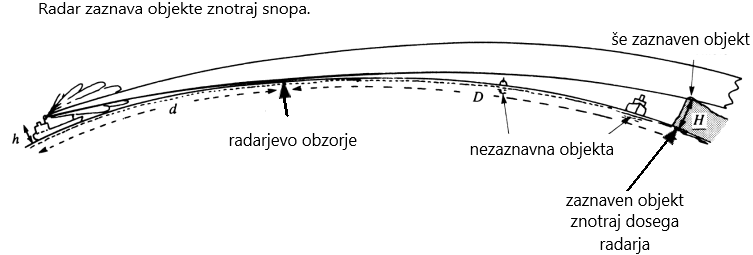
\includegraphics[height=4.5cm]{Predavanja/06_DolocTujegaPolozaja/figs/RadarjevoObzorjeInDoseg.png}
	\caption{Radarsko obzorje je določeno s pogoji atmosfere, doseg radarja pa z lastnostmi snopa in antene ter z lastnostmi objektov.}
	\label{fig:RadarObzorjeDoseg}       % Give a unique label
\end{figure} 
%


%DOC http://www.furuno.com/en/products/radar
radar, SAR
določanje razdalje do objekta
%http://www.radartutorial.eu/01.basics/Distance-determination.en.html
določanje azimuta objekta
%http://www.radartutorial.eu/01.basics/Direction-determination.en.html
največja enoumno določljiva razdalja
%http://www.radartutorial.eu/01.basics/Maximum%20Unambiguous%20Range.en.html
razdalja do najbližje zaznavnega objekta
%http://www.radartutorial.eu/01.basics/Minimal%20Measuring%20Range.en.html
razločljivost po razdalji
%http://www.radartutorial.eu/01.basics/Range%20Resolution.en.html
točnost določanja tujega položaja
%http://www.radartutorial.eu/01.basics/Radars%20Accuracy.en.html

NOAA radar
%http://player.slideplayer.com/16/5227228/#

Ali fizična velikost odsevnika vpliva na možnost zaznavanja plovil.
Če ima ladja večjo efektivno odsevno površino (v ta parameter pade fizična velikost, material, oblika, relativna usmerjenost glede na os radarske antene), je možnost zaznavanja ladje večja.


\section{Section Heading}
\label{sec:1}
% Always give a unique label
% and use \ref{<label>} for cross-references
% and \cite{<label>} for bibliographic references
% use \sectionmark{}
% to alter or adjust the section heading in the running head
Your text goes here. Use the \LaTeX\ automatism for your citations
\cite{monograph}.

\subsection{Subsection Heading}
\label{sec:2}
Your text goes here.

\begin{equation}
\vec{a}\times\vec{b}=\vec{c}
\end{equation}

\subsubsection{Subsubsection Heading}
Your text goes here. Use the \LaTeX\ automatism for cross-references as
well as for your citations, see Sect.~\ref{sec:1}.

\paragraph{Paragraph Heading} %
Your text goes here.

\subparagraph{Subparagraph Heading.} Your text goes here.%
%
\index{paragraph}
% Use the \index{} command to code your index words
%
% For tables use
%
\begin{table}
\centering
\caption{Please write your table caption here}
\label{tab:1}       % Give a unique label
%
% For LaTeX tables use
%
\begin{tabular}{lll}
\hline\noalign{\smallskip}
first & second & third  \\
\noalign{\smallskip}\hline\noalign{\smallskip}
number & number & number \\
number & number & number \\
\noalign{\smallskip}\hline
\end{tabular}
\end{table}
%
%
% For figures use
%
\begin{figure}
\centering
% Use the relevant command for your figure-insertion program
% to insert the figure file.
% For example, with the option graphics use

\includegraphics[height=4cm]{figure}
%
% If not, use
%\picplace{5cm}{2cm} % Give the correct figure height and width in cm
%
\caption{Please write your figure caption here}
\label{fig:1}       % Give a unique label
\end{figure}
%
% For built-in environments use
%
\begin{theorem}
Theorem text goes here.
\end{theorem}
%
% or
%
\begin{lemma}
Lemma text goes here.
\end{lemma}
%
%
% Problems or Exercises should be sorted chapterwise
\section*{Vprašanja v razmislek in poglobitev}
\addcontentsline{toc}{section}{Problems}
%
% Use the following environment.
% Don't forget to label each problem;
% the label is needed for the solutions' environment
\begin{prob}
\label{prob1.ZaznavanjeRadarja}
\textbf{Omejitve zaznavanja z radarjem}\\
(a) Koliko mikrosekund bo radarski signal potreboval do 6NM oddaljenega objekta in nazaj?\\
(b) Na koliko navtičnih milj bi lahko ladijski radar enoumno zaznaval objekte, če ima nastavljeno frekvenco ponavljanja impulzov ($f_{PR}$) na 3000 Hz? Koliko mora nastaviti  $f_{PR}$, da bo enoumno določal oddaljenosti objektov do 24NM? \\
(c) Plovilo je opremljeno z radarjem z dosegom 32 NM.  Radarska antena je na plovilu nameščena na višini 35,0 metrov nad gladino morja. Plovilo se približuje skalnati obali s stenami visokimi 7,0 m. Pojasnite na katerih oddaljenostih od obale je možno pričakovati, da se bo skalnata obala pojavila na radarskemu zaslonu? \\
(č) Od česa je odvisna najmanjša razdalja odkrivanja? Od česa je odvisen najmanjši doseg radarja? Izračunaj najmanjši doseg, če sega $H_{antene}$ = 25m nad gladino, širina snopa v vertikalni ravnini $23^{\circ}$.\\
(d) Koliko znaša najmanjša zaznavna razdalja radarja, če je čas vzpostavitve TR stikala 1,5 mikrosekunde, čas trajanja impulzov pa 0,5 mikrosekunde?
\end{prob}

\begin{prob}
\label{prob2.Odkrivanje}
\textbf{Meje odkrivanja}\\
(a) \\
(b) The second part of the problem is described here.
\end{prob}



%
